\subsection{Power and Temperature}
Accounting for power and temperature is key to achieving effectiveness,
efficiency, and robustness. However, power consumption and heat dissipation are
a result of a myriad of interactions between numerous hardware and software
components comprising modern electronic systems. It is, therefore, difficult to
describe mathematically or algorithmically the impact of a parameter on the
power and temperature characteristics of the system being developed. Moreover,
many aspects of the system are inherently uncertain to the designer. One of the
reasons is process variation \cite{chandrakasan2000}: the properties of
fabricated dies deviate from the nominal ones since process parameters cannot be
controlled precisely using the technologies currently employed in the
fabrication process. Another reason is aging \cite{coskun2006}: the performance
of a system degrades over time due to natural or accelerated wear, which is
unlikely to be uniform. Yet another and perhaps the most consequential reason is
workload: the demand on a system in the field is rarely, if ever, known in the
lab. Such uncertainties inevitably make power and temperature characteristics of
electronic systems uncertain as well.

The above concerns are particularly hard to address from a theoretical
standpoint. They can be better dealt with taking a more pragmatic approach,
namely, making use of on-chip\footnote{In this paper, we use \emph{on-chip},
\emph{online}, and \emph{runtime} interchangeably.} data. To elaborate, assuming
that the system at hand provides basic profiling and monitoring mechanisms such
as hardware performance counters and thermal sensors, which is typically the
case, direct or indirect power and temperature readings are an invaluable source
of information for making power- and temperature-aware decisions. The
attractiveness of the on-chip-data route is due to the fact that only one
particular fabricated hardware in one particular environment needs to be
considered. More importantly, being on the chip enables adaptation, which can
also be made continuous. This means that instances of the system are treated on
a case-by-case basis; each instance attains a custom-built, fine-tuned solution,
and this solution evolves over time, diligently following any changes.

\subsection{Proactive Management}
\begin{figure}
  \centering
  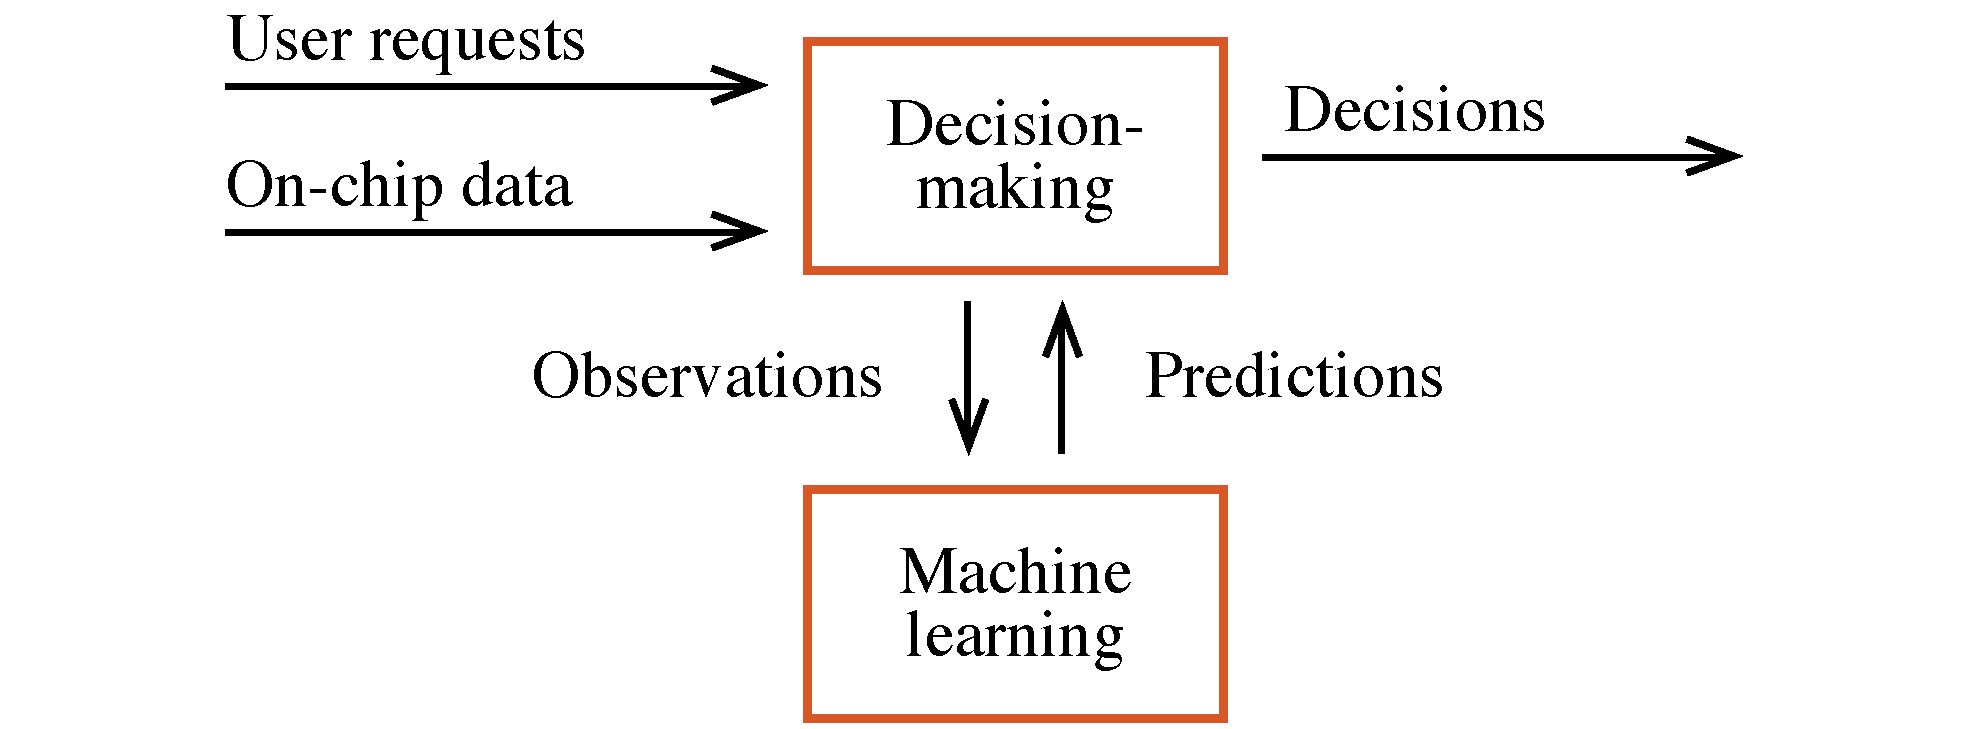
\includegraphics[width=1.0\columnwidth]{include/assets/figures/governor.pdf}

  \caption{A proactive governor of an electronic system. \emph{Observations}
  refers to the data used for learning. \emph{Predictions} refers to the data
  that the management strategy needs to know in advance in order to make
  proactive decisions.}

  \flab{governor}
\end{figure}

Power and temperature data should be available in a timely manner. Proactive
management strategies, which we shall also refer to as proactive governors, are
known to be more efficient than reactive ones since they aim at preventing
problems instead of recovering from the consequences of problems
\cite{coskun2008, chaudhry2015}, which, in particular, avoids slowing or
shutting down processing elements. Acting proactively requires peaking into the
future or, more formally, being able to forecast future behavior. Consequently,
the first step towards proactive power- and temperature-aware management---and,
hence, towards making electronic products more reliable and energy
efficient---is to predict the power consumption and heat dissipation.

Predicting the future relies on learning from the past. This task is typically
accomplished by virtue of tools from statistics and adjacent fields such as
machine learning \cite{bishop2006}. In this case, a proactive governor contains
a learning component, which assimilates relevant on-chip data and makes
predictions. An illustration of this scenario is given in \fref{governor}. To
give a concrete example, in \cite{coskun2008}, temperature forecasting is based
on an autoregressive moving-average model, enabling the development of an
efficient thermal management strategy for multiprocessor systems. Another
example is the work presented in \cite{kumar2010}, which aims at aiding runtime
thermal management of multiprocessor systems by developing an on-chip
temperature predictor based on artificial neural networks.

In the above, we have argued for the usage of learning-based techniques for the
management of electronic systems, and we have put emphasis on those techniques
that learn online, that is, at runtime on the chip, as they are capable of
adaptation. However, the present work is not concerned with the development of
any particular technique of this kind. Instead, the goal of our work is to
provide an infrastructure that facilitates the development of such techniques,
and this infrastructure addresses the following major concern.

\subsection{Data for Learning} \slab{simulation}
\begin{figure}
  \centering
  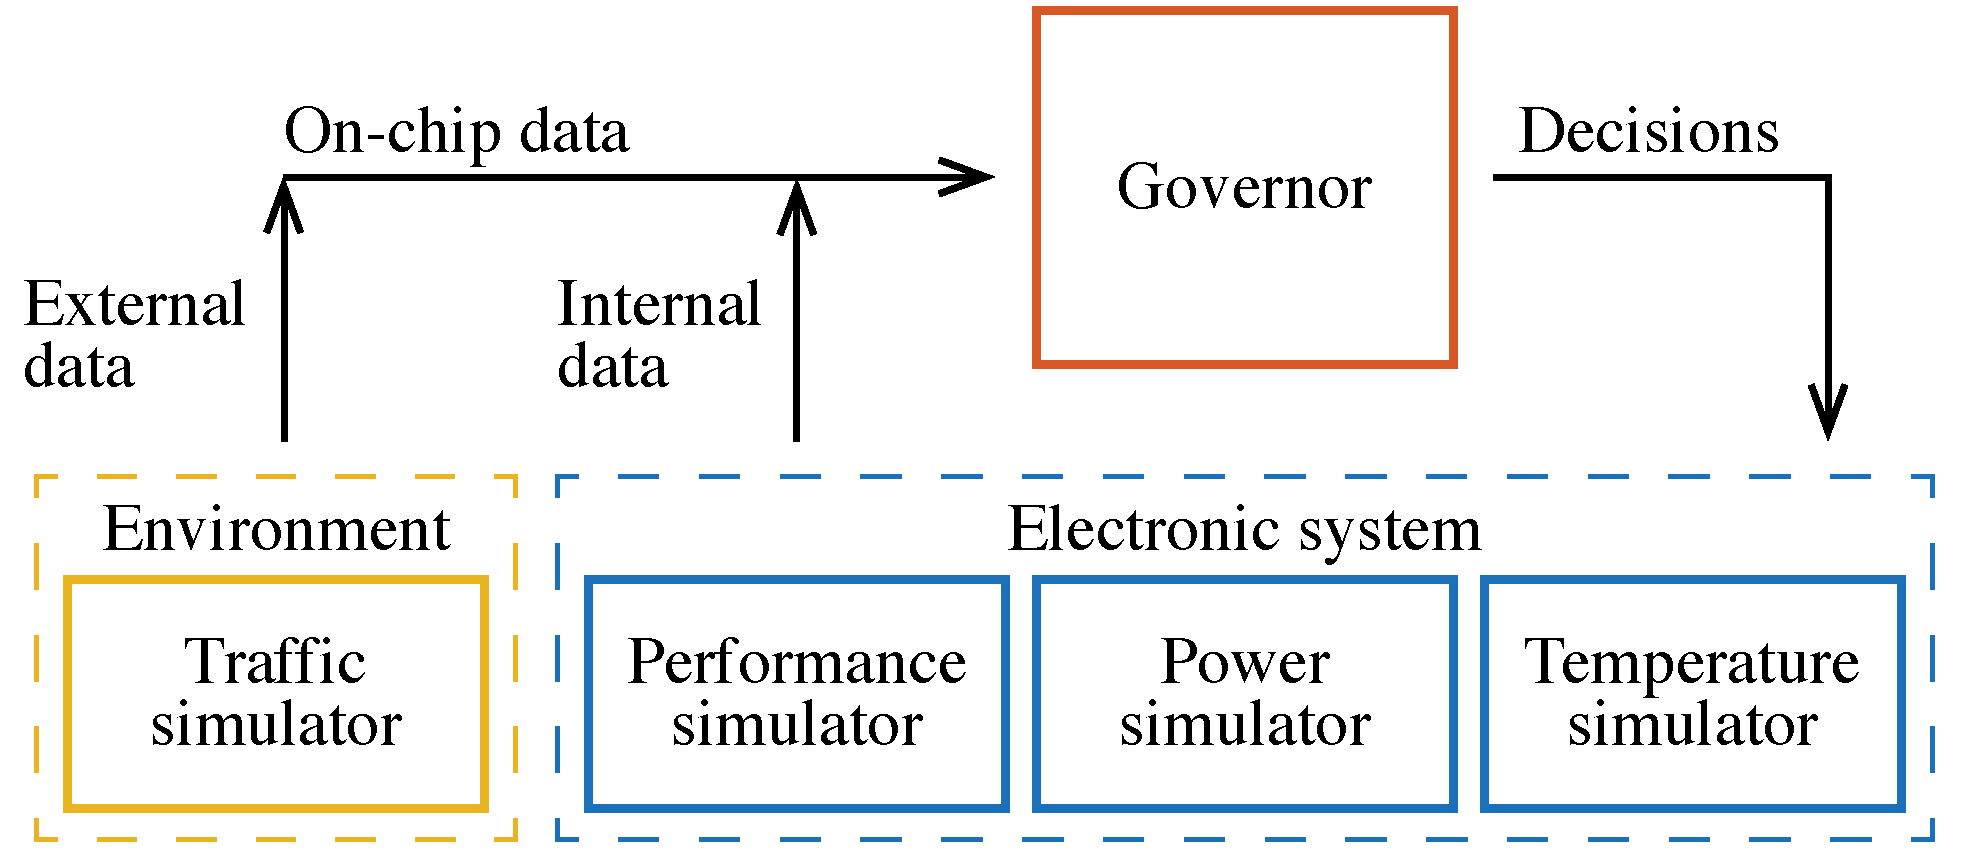
\includegraphics[width=1.0\columnwidth]{include/assets/figures/development.pdf}

  \caption{An experimental setup for developing management strategies
  (governors). \emph{Online data} refers to the data available on the chip
  regardless of their origin. The right dashed box should be understood at a
  single module, and the corresponding arrows should be treated accordingly.}

  \flab{development}
\end{figure}

Regardless of the learning tool utilized, the tool needs data to learn from.
Prior to a physical instantiation of the platform under consideration, all the
hope rests on the shoulders of computer models and simulators. The need for
simulators is not any lower even when an existing platform is concerned. The
platform might not be available to the interested party, or it might not be an
appropriate place for early experimentation and fluid exploration, which is
arguably the most common scenario in research. In such cases, computer
simulators are of great help, and their ubiquitous usage speaks to this
assertion. Therefore, a typical research environment used for developing a
governor of an electronic system is composed of a number of simulators,
providing data to and processing data from the governor. An illustration of such
an environment, emphasizing power and temperature, is given in
\fref{development} wherein the Governor module is the one depicted in
\fref{governor}, and the purpose of the other modules will be made clear later
on.

Simulations can be undertaken on different levels, depending on the goal in
mind. In order to be useful for learning purposes, simulations should be
sufficiently detailed so that they capture well the traits of real systems.
Although detailed simulations (down to cycle accuracy) are practical for the
design of individual components, such simulations fall short when it comes to
large systems. A modern multiprocessor system is reasonably complex, and it
might take days for a state-of-the-art simulator (not even cycle accurate) to
simulate a short, in wall-clock time, program running on such a system. This
scheme is not affordable for designing data-driven techniques as they require
many simulations with potentially large payloads.

The conclusion to draw is that real data are rarely available, and simulation
data are prohibitively time consuming to obtain. Both are severely limiting from
the standpoint of a researcher trying to leverage the rich machinery of machine
learning. The need for alternative sources of high-quality data fuel is
prominent, and providing such an alternative source is exactly to the goal of
this work. More concretely, we are to build a highly responsive (time-wise)
research infrastructure, which is supposed to be used for the development of
on-chip, data-driven, power- and temperature-aware solutions for multiprocessor
systems instead of the one depicted in \fref{development}.
